\documentclass[10pt]{beamer}
\usefonttheme{professionalfonts}
%\usetheme{Rochester}
%\usetheme{AnnArbor}
\usetheme{Szeged}
\useoutertheme{infolines}
\usecolortheme{dolphin}
\usepackage{graphicx}
% \usepackage[english]{babel}
\usepackage{multicol}
\usepackage{color}
%\usepackage{smartdiagram}


%\definecolor{carmine}{rgb}{0.59, 0.0, 0.09}
\usepackage{amsmath}

\usepackage{graphicx}
\usepackage{tikz}
\usetikzlibrary{shapes.callouts}
\usepackage{multirow}

\usepackage[utf8]{inputenc}

\usepackage{enumerate}
\usepackage[shortlabels]{enumitem}
\usepackage{amsmath,amsthm,amssymb,amsfonts,mathrsfs,latexsym,stmaryrd}
\usepackage{tcolorbox}

\usepackage{color}
\usepackage{amssymb, amsmath, amsbsy}
\usepackage{adjustbox,lipsum}
\usepackage{placeins}

\usepackage{textpos}
\usepackage{wrapfig}
\usepackage[spanish, es-tabla]{babel}

\usepackage{caption}
\setlength{\parindent}{15pt}
\hypersetup{hyperfootnotes=false}

\usepackage{url}
\usepackage{float}
\usepackage{tikz}
\usetikzlibrary{patterns}


\title[ICS-294]{Econometría ICS-294\\ \small{Clase 4: Variables omitidas}}

\author{Francisco Alfaro Medina}
\institute[USM]
{Universidad Técnica Federico Santa María\\ % Your institution for the title page
	\medskip
	\textit{francisco.alfaro@usm.cl} % Your email address

}
\logo{

\includegraphics[width=3cm]{Figuras/logoUSM.png}
}
\date{}
\newcommand\Fontvi{\fontsize{9}{7.2}\selectfont}
\begin{document}

\begin{frame}
	\titlepage % Print the title page as the first slide
\end{frame}

\begin{frame}{Objetivos de la Clase}

Al finalizar esta clase, el estudiante será capaz de:

\begin{itemize}
    \item[\checkmark] Reconocer el supuesto clave de MCO para causalidad: $E[\varepsilon\mid x]=0$.
    \item[\checkmark] Derivar la \textbf{fórmula del sesgo por variable omitida} $\tilde\beta_1=\beta_1+\beta_2\delta_1$.
    \item[\checkmark] Determinar el \textbf{signo} del sesgo a partir de $\beta_2$ y $\delta_1$.
    \item[\checkmark] Entender por qué incluir variables irrelevantes no sesga pero \textbf{aumenta la varianza}.
    \item[\checkmark] Aplicar el diagnóstico a casos reales (tabaquismo, retornos a la educación).
\end{itemize}

\end{frame}

\begin{frame}{Sesgo de selección y MCO}
    \begin{itemize}
               \item Supongamos que tenemos el siguiente modelo lineal donde nos interesa el efecto de $x_{i}$ en $y_{i}$.
        $$
        y_{i}=\alpha+\beta x_{i}+\varepsilon_{i}
        $$
        \item El supuesto cl\'asico crucial de MCO para que $\beta$ sea el efecto causal (no haya sesgo de selección) es que:
        $$
        E\left[\epsilon \mid x\right]=0
        $$
        \item Es decir, que todo lo que esta en el error no correlaciona con x.
        \item Si esto no se cumple, nuestro coeficiente estar\'a sesgado.
    \end{itemize}
\end{frame}

\begin{frame}{Sesgo por Variables omitidas}
    \begin{itemize}
        \item ¿Qué pasa si omitimos una variable que afecta a $x$?
        \item ¿En t\'erminos de grupo tratamiento y control, que pasa si omitimos una variable que determina si el individuo es tratado o no?
        \item En este caso, no se cumple que $E\left[\epsilon \mid x\right]=0$ y vamos a tener sesgo de selecci\'on.
        \item Ejemplo: quiero estudiar el efecto de la consultor\'ia en la productividad de la empresa. Sea $x_{i}$ una variable binaria que toma valor 1 si la empresa recibi\'o asesoramiento por la consultora.
        $$
        \text{productividad}_{i}=\alpha+\beta \cdot x_{i}+\epsilon_{i}
        $$
        \item es el $\hat{\beta}$ estimado por OLS el efecto causal? Qu\'e variables estoy omitiendo?
        \item Podemos pensar que en el error est\'a el tamaño de la empresa. Solo empresas m\'as grandes pueden pagar por consultor\'ia. Es decir, el tamaño correlaciona positivamente con la x. Al estar en el error, nuestro $\hat{\beta}$ MCO estar\'a sesgado.
    \end{itemize}
\end{frame}

\begin{frame}{Omitiendo variables}
    \begin{itemize}
        \item Suponga que la población sigue la siguiente ecuación (verdadera),
        \begin{equation*}
            y=\alpha+ \beta_{1}x_{1}+\beta_{2} x_{2}+u \tag{A}
        \end{equation*}
        donde $E[u \mid x]=0$.
        \item (auxiliar) Ademas, supongan que sabemos que $x_{2}$ esta relacionada con $x_{1}$ de la siguiente manera:

        \begin{equation*}
        x_{2}=\delta_{0}+\delta_{1} x_{1}+v \tag{B}
        \end{equation*}

        \item Supongamos que como no observamos $x_{2}$, estimamos el modelo MCO omitiendola (mandandola al error):
        \begin{equation*}
        y=\tilde{\alpha}+x_{1} \tilde{\beta}_{1}+\epsilon \tag{C}
        \end{equation*}
        \item ¿Qué supuesto no se cumpliría en este caso?
        \item Noten que comparando con (A), sabemos que $\epsilon=\beta_{2} x_{2}+u$. Por (B), sabemos que $x_{1}$ correlaciona con $x_{2}$, entonces no se cumple $E\left[\epsilon \mid x_{1}\right]=0$.
        \item Entonces, ¿qué esta capturando $\tilde{\beta}_{1}$?
    \end{itemize}
\end{frame}

\begin{frame}{Omitiendo variables}
    \begin{itemize}
        \item Reemplazando (B) en (A):
        $$
        y=\alpha+x_{1} \beta_{1}+\beta_{2}\left(\delta_{0}+\delta_{1} x_{1}+v\right)+u
        $$
        \item Reordenando:
        $$
        y=\left(\alpha+\beta_2\delta_{0}\right)+x_{1}\left(\beta_{1}+\beta_{2} \delta_{1}\right)+\left(u+\beta_{2} v\right)
        $$
        \item Es decir, que cuando omitimos una variable y estimamos un modelo como (C). El coeficiente que estimamos es:
        $$
        \tilde{\beta}_{1}=\beta_{1}+\beta_{2} \delta_{1}
        $$
        \item Entonces, capturamos el efecto causal $\left(\beta_{1}\right)$ y un sesgo dado por $\beta_{2} \delta_{1}$.
        \item ¿De qué depende el sesgo? ¿Cuándo es 0?
    \end{itemize}
\end{frame}

% ===================== TEOREMA CLAVE DE LA CLASE =====================

\begin{frame}[allowframebreaks]{Teorema: sesgo por variable omitida (derivación con esperanzas)}

\begin{alertblock}{Proposición (Omitted Variable Bias)}
Sea el modelo verdadero $y=\beta_0+\beta_1 x_1+\beta_2 x_2+u$ con $E[u\mid x_1,x_2]=0$. Si estimamos por MCO la regresión \emph{corta} $y=\tilde\beta_0+\tilde\beta_1 x_1+\epsilon$ (omitiendo $x_2$), entonces
\[
E[\tilde\beta_1] = \beta_1 + \beta_2\,\delta_1,
\qquad
\delta_1=\frac{\text{Cov}(x_1,x_2)}{\text{Var}(x_1)},
\]
donde $\delta_1$ es la pendiente de la regresión auxiliar de $x_2$ sobre $x_1$.
\end{alertblock}

\begin{exampleblock}{Demostración}
\textbf{Paso 1.} El estimador MCO de pendiente en la regresión corta es
\[
\tilde\beta_1=\frac{\sum_i (x_{1i}-\bar x_1)(y_i-\bar y)}{\sum_i (x_{1i}-\bar x_1)^2}
=\frac{\widehat{\text{Cov}}(x_1,y)}{\widehat{\text{Var}}(x_1)}.
\]

\textbf{Paso 2.} Sustituimos el modelo verdadero $y=\beta_0+\beta_1 x_1+\beta_2 x_2+u$ en la covarianza. Usando que la covarianza es lineal y que $\text{Cov}(x_1,\text{constante})=0$:
\[
\text{Cov}(x_1,y)=\beta_1\,\text{Var}(x_1)+\beta_2\,\text{Cov}(x_1,x_2)+\text{Cov}(x_1,u).
\]

\framebreak

\textbf{Paso 3.} Dividiendo por $\text{Var}(x_1)$ y tomando esperanza (en muestras grandes, o condicional a $x$):
\[
E[\tilde\beta_1]=\beta_1+\beta_2\,\underbrace{\frac{\text{Cov}(x_1,x_2)}{\text{Var}(x_1)}}_{=\,\delta_1}+\underbrace{\frac{\text{Cov}(x_1,u)}{\text{Var}(x_1)}}_{=\,0}.
\]
El último término es $0$ porque $E[u\mid x_1,x_2]=0\Rightarrow \text{Cov}(x_1,u)=0$.

\textbf{Paso 4.} Por lo tanto
\[
\boxed{\,E[\tilde\beta_1]=\beta_1+\beta_2\,\delta_1\,}.
\]
El término $\beta_2\,\delta_1$ es el \textbf{sesgo}. \hfill $\square$
\end{exampleblock}

\begin{block}{¿Cuándo el sesgo es cero?}
El sesgo $\beta_2\delta_1=0$ si y solo si (i) $\beta_2=0$ ($x_2$ no afecta a $y$, es irrelevante), o (ii) $\delta_1=0$ ($x_2$ no correlaciona con $x_1$). \emph{Basta} con una de las dos.
\end{block}

\end{frame}

\begin{frame}
    \frametitle{Sesgo por omisión de variable}
    \begin{columns}
        \column{0.5\textwidth}
        % Columna de diagramas
        \begin{enumerate}
            \item[{\color{blue}1)}]
        \begin{figure}[h]
            \centering
            \begin{tikzpicture}[->, thick]
                \node (X1a) at (0,0) {$X1$};
                \node (Ya) at (2,0) {$Y$};
                \node (X2a) at (1,-1) {$X2$};
                \draw[brown] (X1a) -- (Ya);
                \draw[red] (X2a) -- (Ya) node[midway, right] {\textcolor{red}{$\beta_2$}};
            \end{tikzpicture}
        %    \caption{Diagrama 1}
        \end{figure}
    \item[{\color{blue}2)}]
        \begin{figure}[h]
            \centering
            \begin{tikzpicture}[->, thick]
                \node (X1b) at (0,0) {$X1$};
                \node (Yb) at (2,0) {$Y$};
                \node (X2b) at (1,-1) {$X2$};
                \draw[brown] (X1b) -- (Yb);
                \draw[red] (X2b) -- (X1b) node[midway, left] {\textcolor{red}{$\delta$}};
            \end{tikzpicture}
          %  \caption{Diagrama 2}
        \end{figure}
       \item[{\color{blue}3)}]
               \begin{figure}[h]
            \centering
            \begin{tikzpicture}[->, thick]
                \node (X1c) at (0,0) {$X1$};
                \node (Yc) at (2,0) {$Y$};
                \node (X2c) at (1,-1) {$X2$};
                \draw[brown] (X1c) -- (Yc);
                \draw[red] (X2c) -- (X1c) node[midway, left] {\textcolor{red}{$\delta$}};
                \draw[red] (X2c) -- (Yc) node[midway, right] {\textcolor{red}{$\beta_2$}};
            \end{tikzpicture}
            %\caption{Diagrama 3}
        \end{figure}
        \end{enumerate}
        \column{0.5\textwidth}
        % Columna de texto explicativo
        \begin{itemize}
        \item Cuando una variable omitida provocar\'a un sesgo entonces?
        $$
        \tilde{\beta}_{1}=\beta_{1}+\beta_{2} \delta_{1}
        $$
        % \begin{figure}
        %     \centering
        %     
\includegraphics[width=0.4\linewidth]{z SebastianG/Imagenes/Grafico2_1.jpeg}
        % \end{figure}
        \item Solo en el caso (3) tenemos sesgo. Cuando omitimos una variable que afecta a X y a Y al mismo tiempo (en general lo segundo siempre pasa).
        \item Ejemplo:\\
        $X_{1}$ : educacion, $Y=$ salario, \\
        $x_{2}$ : Inteligencia. En ese caso, $\beta_{2}>0$, $\delta_{1}>0$. Por lo que $\tilde{\beta}_{1}$ sobre-estimar\'a el verdadero valor del par\'ametro.
    \end{itemize}
    \end{columns}
\end{frame}

\begin{frame}{Sesgo por omisión de variable}
    $$
    \tilde{\beta}_{1}=\beta_{1}+\beta_{2} \delta_{1}
    $$
    \begin{itemize}
        \item Pensando en los signos de $\beta_{2}$ (como afecta la omitida a y) y $\delta_{1}$ (como afecta la omitida a $x_{1}$ ), podemos comprender la direccion del sesgo. (los ejemplos con regresi\'on de educaci\'on y salario)
        \begin{enumerate}
            \item Si $\delta_{1}>0, \beta_{2}>0$ : Sesgo positivo. Ejemplo omitida: Inteligencia.
            \item Si $\delta_{1}<0, \beta_{2}<0$ : Sesgo positivo.
            \item $\delta_{1}<0, \beta_{2}>0$ : Sesgo negativo.
            \item $\delta_{1}>0, \beta_{2}<0$ : Sesgo negativo.
        \end{enumerate}

        \item La intuici\'on es f\'acil. Piensen el caso (1). La gente mas inteligente va m\'as a la universidad $\left(\delta_{1}>0\right) y$, adem\'as, la inteligencia mejora tu salario ( $\beta_{2}>0$ ). Entonces, al omitir inteligencia, el coeficiente de educaci\'on se captura no solo el efecto causal sino tambi\'en el hecho de que gente mas inteligente va m\'as a la universidad y esa gente gana m\'as (sin importar el efecto de la educaci\'on en si misma).
    \end{itemize}
\end{frame}

\begin{frame}{Tabla resumen: dirección del sesgo}

\begin{center}
\begin{tabular}{c|cc}
 & $\text{Corr}(x_1,x_2)>0$ & $\text{Corr}(x_1,x_2)<0$ \\
 & $(\delta_1>0)$ & $(\delta_1<0)$ \\
\hline
$\beta_2>0$ & Sesgo \textbf{positivo} & Sesgo \textbf{negativo}\\
$\beta_2<0$ & Sesgo \textbf{negativo} & Sesgo \textbf{positivo}\\
\end{tabular}
\end{center}

\vspace{0.4cm}

\begin{itemize}
    \item Sesgo \textbf{positivo} $\Rightarrow$ $\tilde\beta_1$ \emph{sobreestima} $\beta_1$.
    \item Sesgo \textbf{negativo} $\Rightarrow$ $\tilde\beta_1$ \emph{subestima} $\beta_1$.
    \item Regla mnemotécnica: el signo del sesgo es el \textbf{producto} de los signos de $\beta_2$ y $\delta_1$.
\end{itemize}

\end{frame}

\begin{frame}{Soluciones a variables omitidas: Controles}
    \begin{itemize}
        \item Cu\'al es la manera m\'as obvia de solucionar el problema anterior?
        \item Si tengo la variable $x_{2}$, la puedo incluir como control en la regresi\'on y soluciono el problema.
        \item Vuelvo al caso en que $E[u \mid {\bf x}]=0$ porque ahora estoy dejando ceteris paribus $x_{2}$.
        \item En este caso, resuelve el problema porque conozco exacto el modelo verdadero y se que solo omit\'ia $x_{2}$. Sin embargo, muchas veces no alcanza porque hay otras variables omitidas.
    \end{itemize}
\end{frame}

\begin{frame}{Ejemplo 1}
    \begin{itemize}
        \item Appleton, French and Vanderpump (1996): relación entre consumo de cigarillos y muerte.
    \end{itemize}

    %Nota: mejor hacer esto con una imagen nomás
    \begin{figure}
        \centering
        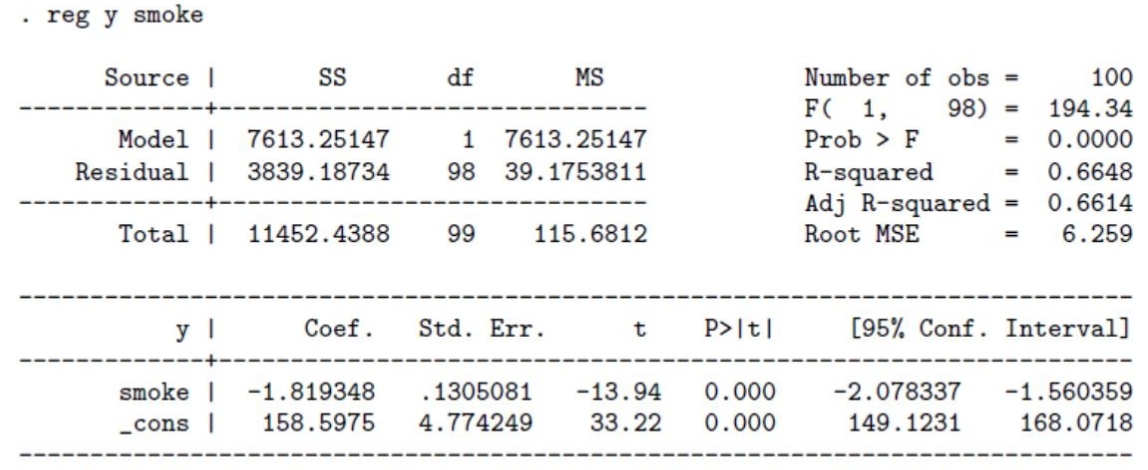
\includegraphics[width=0.8\linewidth]{complemetario/Imagenes/RegySmoke.jpeg}
    \end{figure}
    \begin{itemize}
        \item $\hat{\tilde{\beta}}_{1}=-1.81$
        \item ¿Qué variables estamos omitiendo aca?
    \end{itemize}
\end{frame}

\begin{frame}{Ejemplo 2}
    \begin{itemize}
        \item ¿Y si agregamos edad?
        \begin{figure}
            \centering
            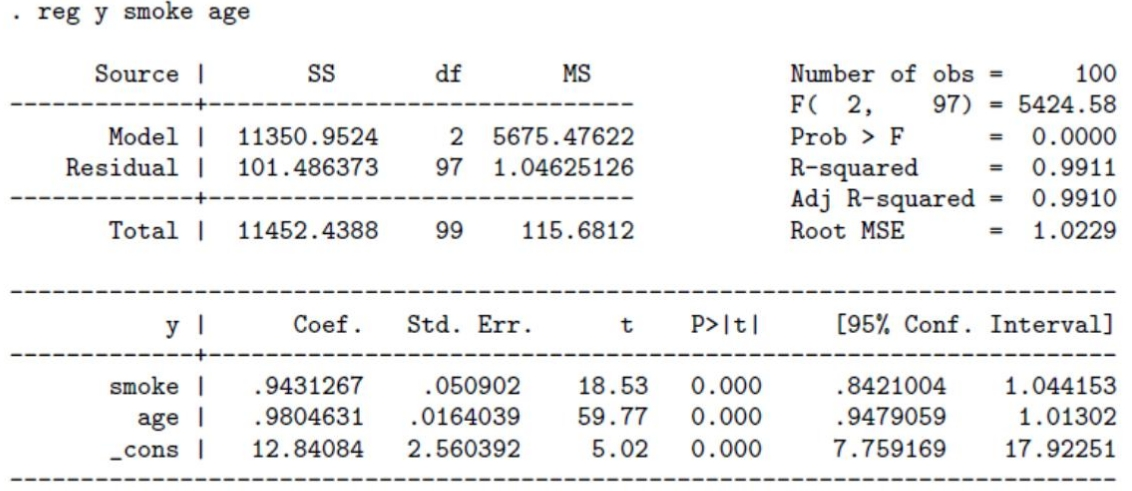
\includegraphics[width=0.8\linewidth]{complemetario/Imagenes/RegySmokeAge.jpeg}
        \end{figure}
    \end{itemize}
    \begin{itemize}
        \item Si este fuera el modelo verdadero, $\hat{\beta}_{1}=0.94>\hat{\tilde{\beta}}_{1}=-1.81$. Si $\hat{\beta}_{2}>0$, ¿qué me dice esto sobre el signo de relaci\'on entre edad y fumar cigarrillos $\delta_{2}$?
        \item Recuerden: $\tilde{\beta}_{1}=\beta_{1}+\beta_{2} \delta_{2}$
        \item Es negativa: cuanto mayor es la persona, menos fuma.
    \end{itemize}
\end{frame}

\begin{frame}{¿Más es mejor?}
    \begin{itemize}
        \item Uno podría pensar que tiene que agregar todas las variables posibles al modelo, para evitar omitir variables.
        \item Sin embargo, esto trae problemas.
        \item Se dice que un modelo está sobreespecificado cuando se incluye en la regresión variables que no forman parte del modelo poblacional.
        \item Incluir variables irrelevantes en el modelo no influye en el insesgamiento de los estimadores, pero  incrementa la varianza de los estimadores.
    \end{itemize}
\end{frame}

\begin{frame}[allowframebreaks]{Proposición: variables irrelevantes -- insesgamiento y varianza}

\begin{alertblock}{Proposición (sobreespecificación)}
Suponga que el modelo verdadero es $y=\beta_0+\beta_1 x_1+u$ (con $\beta_2=0$) pero estimamos el modelo \emph{largo} $y=\hat\beta_0+\hat\beta_1 x_1+\hat\beta_2 x_2+\hat u$ que incluye la variable irrelevante $x_2$. Entonces:
\begin{enumerate}
    \item $\hat\beta_1$ \textbf{sigue siendo insesgado}: $E[\hat\beta_1]=\beta_1$.
    \item Si $x_1$ y $x_2$ están correlacionadas, $\text{Var}(\hat\beta_1)$ \textbf{aumenta}.
\end{enumerate}
\end{alertblock}

\begin{exampleblock}{Demostración (insesgamiento)}
El modelo largo \emph{contiene} al verdadero como caso particular ($\beta_2=0$). MCO sobre el modelo largo es insesgado para \emph{todos} sus coeficientes siempre que se cumpla $E[u\mid x_1,x_2]=0$, lo cual se mantiene aquí porque $u$ es el error del modelo verdadero. En particular $E[\hat\beta_1]=\beta_1$ y $E[\hat\beta_2]=\beta_2=0$. Incluir una variable de más \emph{no} introduce sesgo. \hfill $\square$
\end{exampleblock}

\framebreak

\begin{exampleblock}{Demostración (varianza)}
La varianza del estimador del modelo largo es
\[
\text{Var}(\hat\beta_1)=\frac{\sigma^2}{\sum_i(x_{1i}-\bar x_1)^2\,(1-R_1^2)},
\]
donde $R_1^2$ es el $R^2$ de regresar $x_1$ sobre las demás explicativas (aquí, sobre $x_2$). En la regresión corta (sin $x_2$) la varianza es $\sigma^2/\sum_i(x_{1i}-\bar x_1)^2$, es decir, el mismo numerador con $R_1^2=0$.
\\[4pt]
Como $0\le R_1^2<1$, el factor $1/(1-R_1^2)\ge 1$. Por lo tanto, si $x_1$ y $x_2$ están correlacionadas ($R_1^2>0$),
\[
\text{Var}_{\text{largo}}(\hat\beta_1) > \text{Var}_{\text{corto}}(\tilde\beta_1).
\]
Conclusión: agregar una variable irrelevante \emph{infla la varianza} sin reducir el sesgo. \hfill $\square$
\end{exampleblock}

\begin{block}{Trade-off sesgo--varianza}
\textbf{Omitir} una variable relevante $\Rightarrow$ sesgo. \textbf{Incluir} una irrelevante (correlacionada) $\Rightarrow$ más varianza. La especificación busca equilibrar ambos errores.
\end{block}

\end{frame}

\begin{frame}{Sin sesgo de selección}
    \begin{itemize}
        \item Si tenemos la suerte de tener una aleatorización que nos garantiza que no haya sesgo de selección, ¿importa agregar variables adicionales?
        \item Si $X_{1}$ (o $T_{i}$ en t\'erminos de tratamiento) se determina de forma aleatoria, nos garantiza que $E\left[\epsilon_{i} \mid X_{i}\right]=0$
        \item ¡La correlaci\'on entre cualquier variable no incluida en el modelo y el tratamiento será 0!
        \item Entonces, no necesitamos incluir otras variables en el modelo para evitar sesgos.

    \end{itemize}
\end{frame}

% ===================== EJERCICIOS RESUELTOS =====================

\begin{frame}{Ejercicio Resuelto 1}

\begin{block}{Ejercicio 1 (sesgo en retornos a la educación)}
El modelo verdadero del salario es
\[
\log(\text{salario})=\beta_0+\beta_1\,\text{educ}+\beta_2\,\text{habilidad}+u,
\]
pero \emph{no observamos} habilidad y estimamos la regresión corta. Sabemos:
\begin{itemize}
    \item Más habilidad sube el salario: $\beta_2=0.04>0$.
    \item Más habilidad se asocia con más años de educación: $\delta_1=\text{Cov}(\text{educ},\text{hab})/\text{Var}(\text{educ})=1.5>0$.
\end{itemize}
Si el verdadero retorno es $\beta_1=0.06$, ¿qué valor esperaríamos del MCO corto $E[\tilde\beta_1]$, y en qué dirección sesga?
\end{block}

\pause

\begin{exampleblock}{Solución}
Por la fórmula del sesgo:
\[
E[\tilde\beta_1]=\beta_1+\beta_2\,\delta_1=0.06+(0.04)(1.5)=0.06+0.06=0.12.
\]
El sesgo $\beta_2\delta_1=0.06$ es \textbf{positivo} (producto de dos positivos): el MCO corto reporta $12\%$ de retorno cuando el verdadero es $6\%$, \textbf{sobreestimando} al doble. Parte del ``retorno a la educación'' es en realidad retorno a la habilidad no observada.
\end{exampleblock}

\end{frame}

\begin{frame}{Ejercicio Resuelto 2}

\begin{block}{Ejercicio 2 (signo del sesgo, contexto chileno)}
Se estima el efecto del tamaño del curso sobre el puntaje SIMCE: $\text{SIMCE}=\beta_0+\beta_1\,\text{tamaño}+u$, omitiendo el \textbf{nivel socioeconómico (NSE)} del colegio. Se sabe que (i) cursos más pequeños tienden a estar en colegios de mayor NSE (relación tamaño--NSE negativa) y (ii) mayor NSE eleva el SIMCE. Determine el signo del sesgo en $\tilde\beta_1$.
\end{block}

\pause

\begin{exampleblock}{Solución}
Defina $x_2=$ NSE. Tenemos:
\begin{itemize}
    \item $\beta_2>0$ (NSE sube SIMCE).
    \item $\delta_1=\text{Cov}(\text{tamaño},\text{NSE})/\text{Var}(\text{tamaño})<0$ (cursos grandes $\to$ menor NSE).
\end{itemize}
Sesgo $=\beta_2\,\delta_1=(+)(-)<0$: \textbf{negativo}. El MCO corto \emph{subestima} (hace más negativo de lo real) el efecto del tamaño, atribuyendo al tamaño del curso lo que en parte es efecto del NSE.
\end{exampleblock}

\end{frame}

% ===================== EJERCICIOS PROPUESTOS =====================

\begin{frame}{Ejercicios Propuestos}

\begin{block}{Ejercicio 3 (Propuesto -- rutinario)}
En el modelo $y=\beta_0+\beta_1 x_1+\beta_2 x_2+u$ se omite $x_2$. Si $\beta_2=-2$ y $\delta_1=-0.5$, calcule el sesgo y diga si $\tilde\beta_1$ sobre- o subestima $\beta_1$.
\end{block}

\begin{block}{Ejercicio 4 (Propuesto -- intermedio)}
Un investigador estima el efecto del salario mínimo sobre el empleo y omite el ciclo económico (PIB). Plantee el modelo verdadero, identifique los signos plausibles de $\beta_2$ y $\delta_1$, y prediga la dirección del sesgo.
\end{block}

\begin{block}{Ejercicio 5 (Propuesto -- desafiante)}
Demuestre que cuando se omite una variable relevante \emph{ortogonal} a $x_1$ (es decir $\text{Cov}(x_1,x_2)=0$), $\tilde\beta_1$ es insesgado pero su \emph{varianza estimada} ($s^2/\sum(x_{1i}-\bar x_1)^2$) tiende a ser mayor que en el modelo largo. \emph{Indicación:} compare las estimaciones de $\sigma^2$ de ambos modelos.
\end{block}

\end{frame}

\begin{frame}{Conclusiones}
    \begin{itemize}
        \item Incluir variables a un modelo cambia la interpretación de nuestra variable de interés.
        \item El impacto de la exclusión de una variable relevante depende de la correlación entre la variable de interés y la variable omitida y la relación entre la variable omitida y el outcome.
        \item El supuesto clave de MCO para que no haya sesgo es que $E[\epsilon \mid X]=0$.
               \item Es poco frequente que tengamos TODAS las variables que determinan la asignación y entonces, es poco probable que la inclusión de variables nos permita dar una interpretación causal a una regresión lineal.
    \end{itemize}
\end{frame}

\begin{frame}{Resumen}

\begin{block}{Puntos Clave de la Clase 4}
\begin{enumerate}
    \item El supuesto de exogeneidad $E[u\mid x]=0$ es la condición para insesgamiento de MCO.
    \item Omitir una variable relevante correlacionada con $x_1$ produce sesgo: $\tilde\beta_1=\beta_1+\beta_2\delta_1$.
    \item El \textbf{signo} del sesgo es el producto de los signos de $\beta_2$ y $\delta_1$.
    \item Incluir variables \textbf{irrelevantes} no sesga, pero infla $\text{Var}(\hat\beta_1)$: trade-off sesgo--varianza.
    \item La aleatorización elimina la necesidad de controles para evitar sesgo.
\end{enumerate}
\end{block}

\begin{alertblock}{Para la próxima clase}
Revisar: ¿qué pasa cuando las variables están \textbf{mal medidas}? Error de medición y \textbf{sesgo de atenuación}.
\end{alertblock}

\end{frame}

\end{document}
